\section{Systematic Uncertainties}



\begin{frame}{Handling systematics}

    \begin{itemize}
        \item Statistical uncertainties are calculated using different approaches for the two analyses.
        \item Shape analysis:
        \begin{itemize}
            \smaller
            \item uncertainty is included in fit with nuisance parameters (n.p.);
            \item most uncertainties are accounted for using morphing templates;
            \item MC statistical uncertainty accounted for on a bin-by-bin basis using Barlow-Beeston approach;
            \item the same systematic parameter in all relevant categories are fully correlated;
            \item different systematic parameters are independent before fit. (correlations are generated by the fitting process.)
        \end{itemize}
        
        \item Counting analysis:
        \begin{itemize}
            \smaller
            \item uncertainty accounted for by carrying out measurement with each uncertainty source varied by $\pm 1\sigma$;
            \item results in different trigger and $n_b$ categories are analytically combined by $\chi^2$ assuming:
            \begin{itemize}
            \smaller 
                \item the same source of systematics is fully correlated;
                \item difference sources of systematics is independent.
            \end{itemize}
        \end{itemize}
    \end{itemize}

\end{frame}


\begin{frame}{Sources of systematic uncertainties}
\smaller

    \begin{itemize}
        \item Luminosity (2.5\%).
        \item Cross-section\footnotemark: \ttbar (5\%), \tW (5\%), \zjets (10\%), \wjets (5\%), \gjets (10\%), VV (10\%). 
        
        \item QCD estimation in $\ell\PGth$ and $\ell h$ (25\%).
        \item Gen-level reweightings: PU, top \pt, \WW \pt .
        \item Trigger efficiencies: single muon trigger, single electron trigger.
        \item Object reconstruction:
        \begin{itemize}
        \smaller
            \item muon: identification, isolation, energy scale.
            \item electron: identification, reconstruction, energy scale.
            \item tau: identification, misidentification, energy scale.
            \item jet: energy scale, energy resolution.
            \item btag: tag/mistag.
        \end{itemize}
        \item Tau decay branching fractions: $\PGt \to \Pe$, $\PGt \to \PGm$, $\PGt \to \mathrm{h}$.
        \item Simulation of \ttbar: ISR/FSR, matrix element to parton shower matching (ME-PS), underlying event tuning (UE).
        
    \end{itemize}

\footnotetext[2]{\footnotesize Shape analysis decomposes \ttbar, \wjets, \zjets cross-sections into generator parameters, e.g. PDF, \alpS, $\mu_f$, $\mu_r$, to avoid constraining relevant n.p..}
\end{frame}




\begin{frame}{}
counting analysis
    \centering
    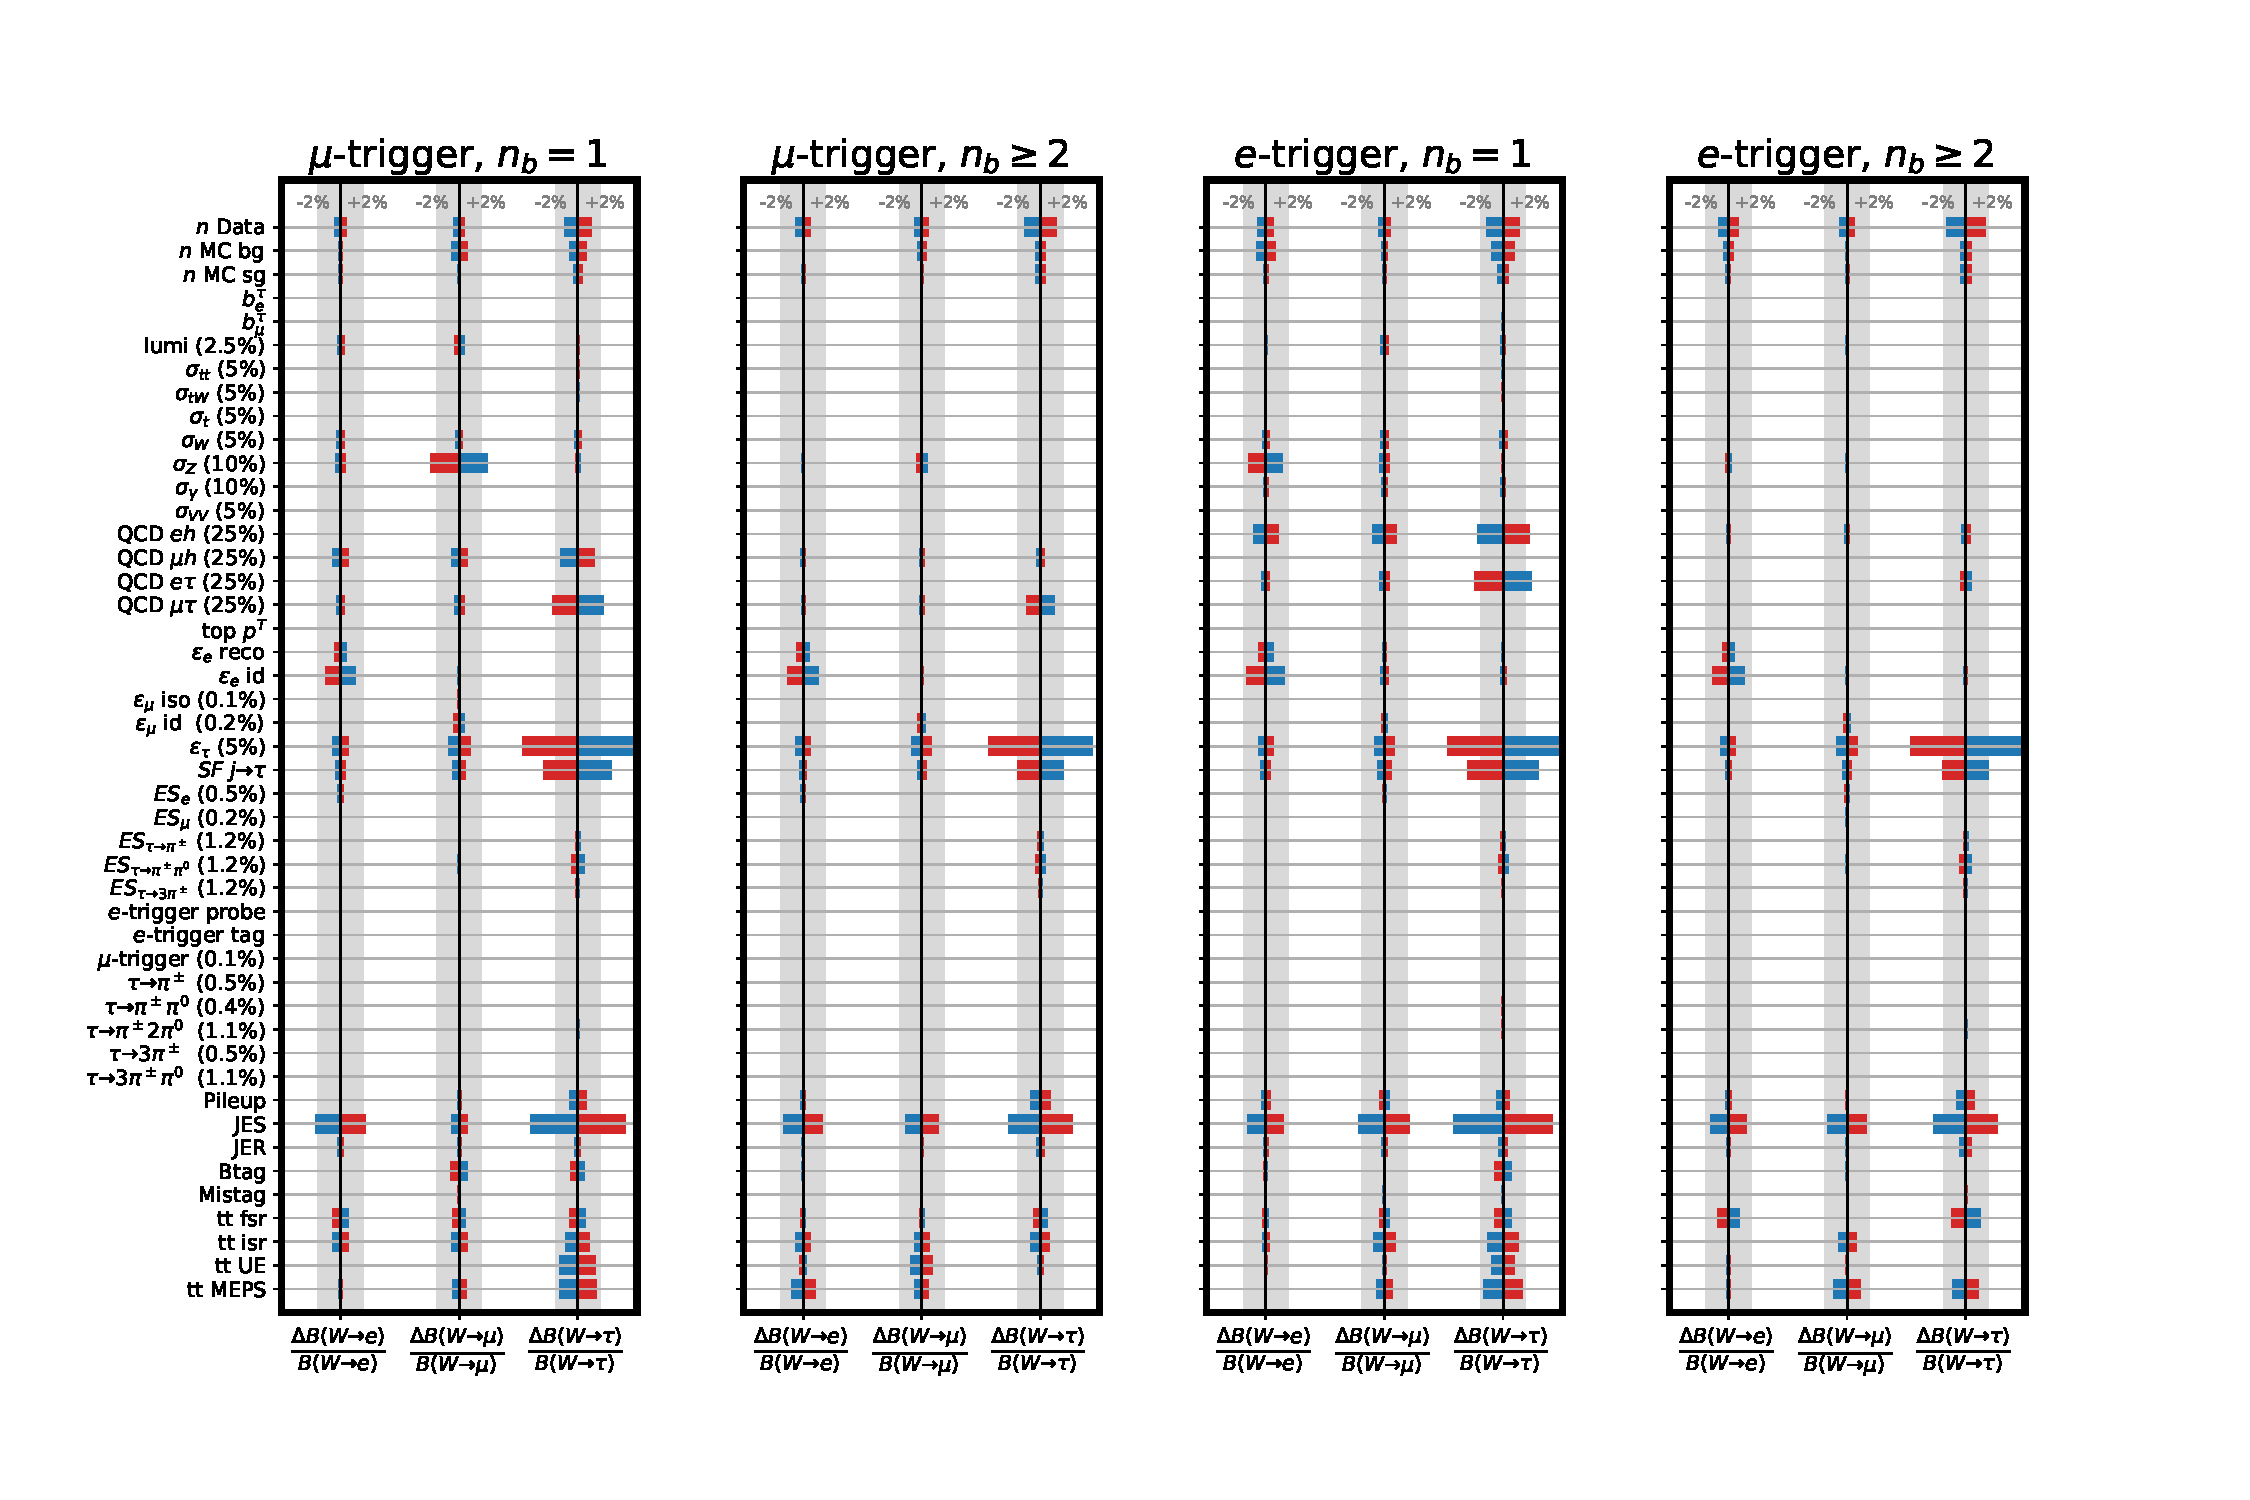
\includegraphics[width=\textwidth, trim=1.5cm 0cm 3.5cm 1cm, clip]{chapters/Analysis/sectionSystematics/figures/systematics_impact_counting.pdf}
\end{frame}

\begin{frame}{}
shape analysis
    \centering
    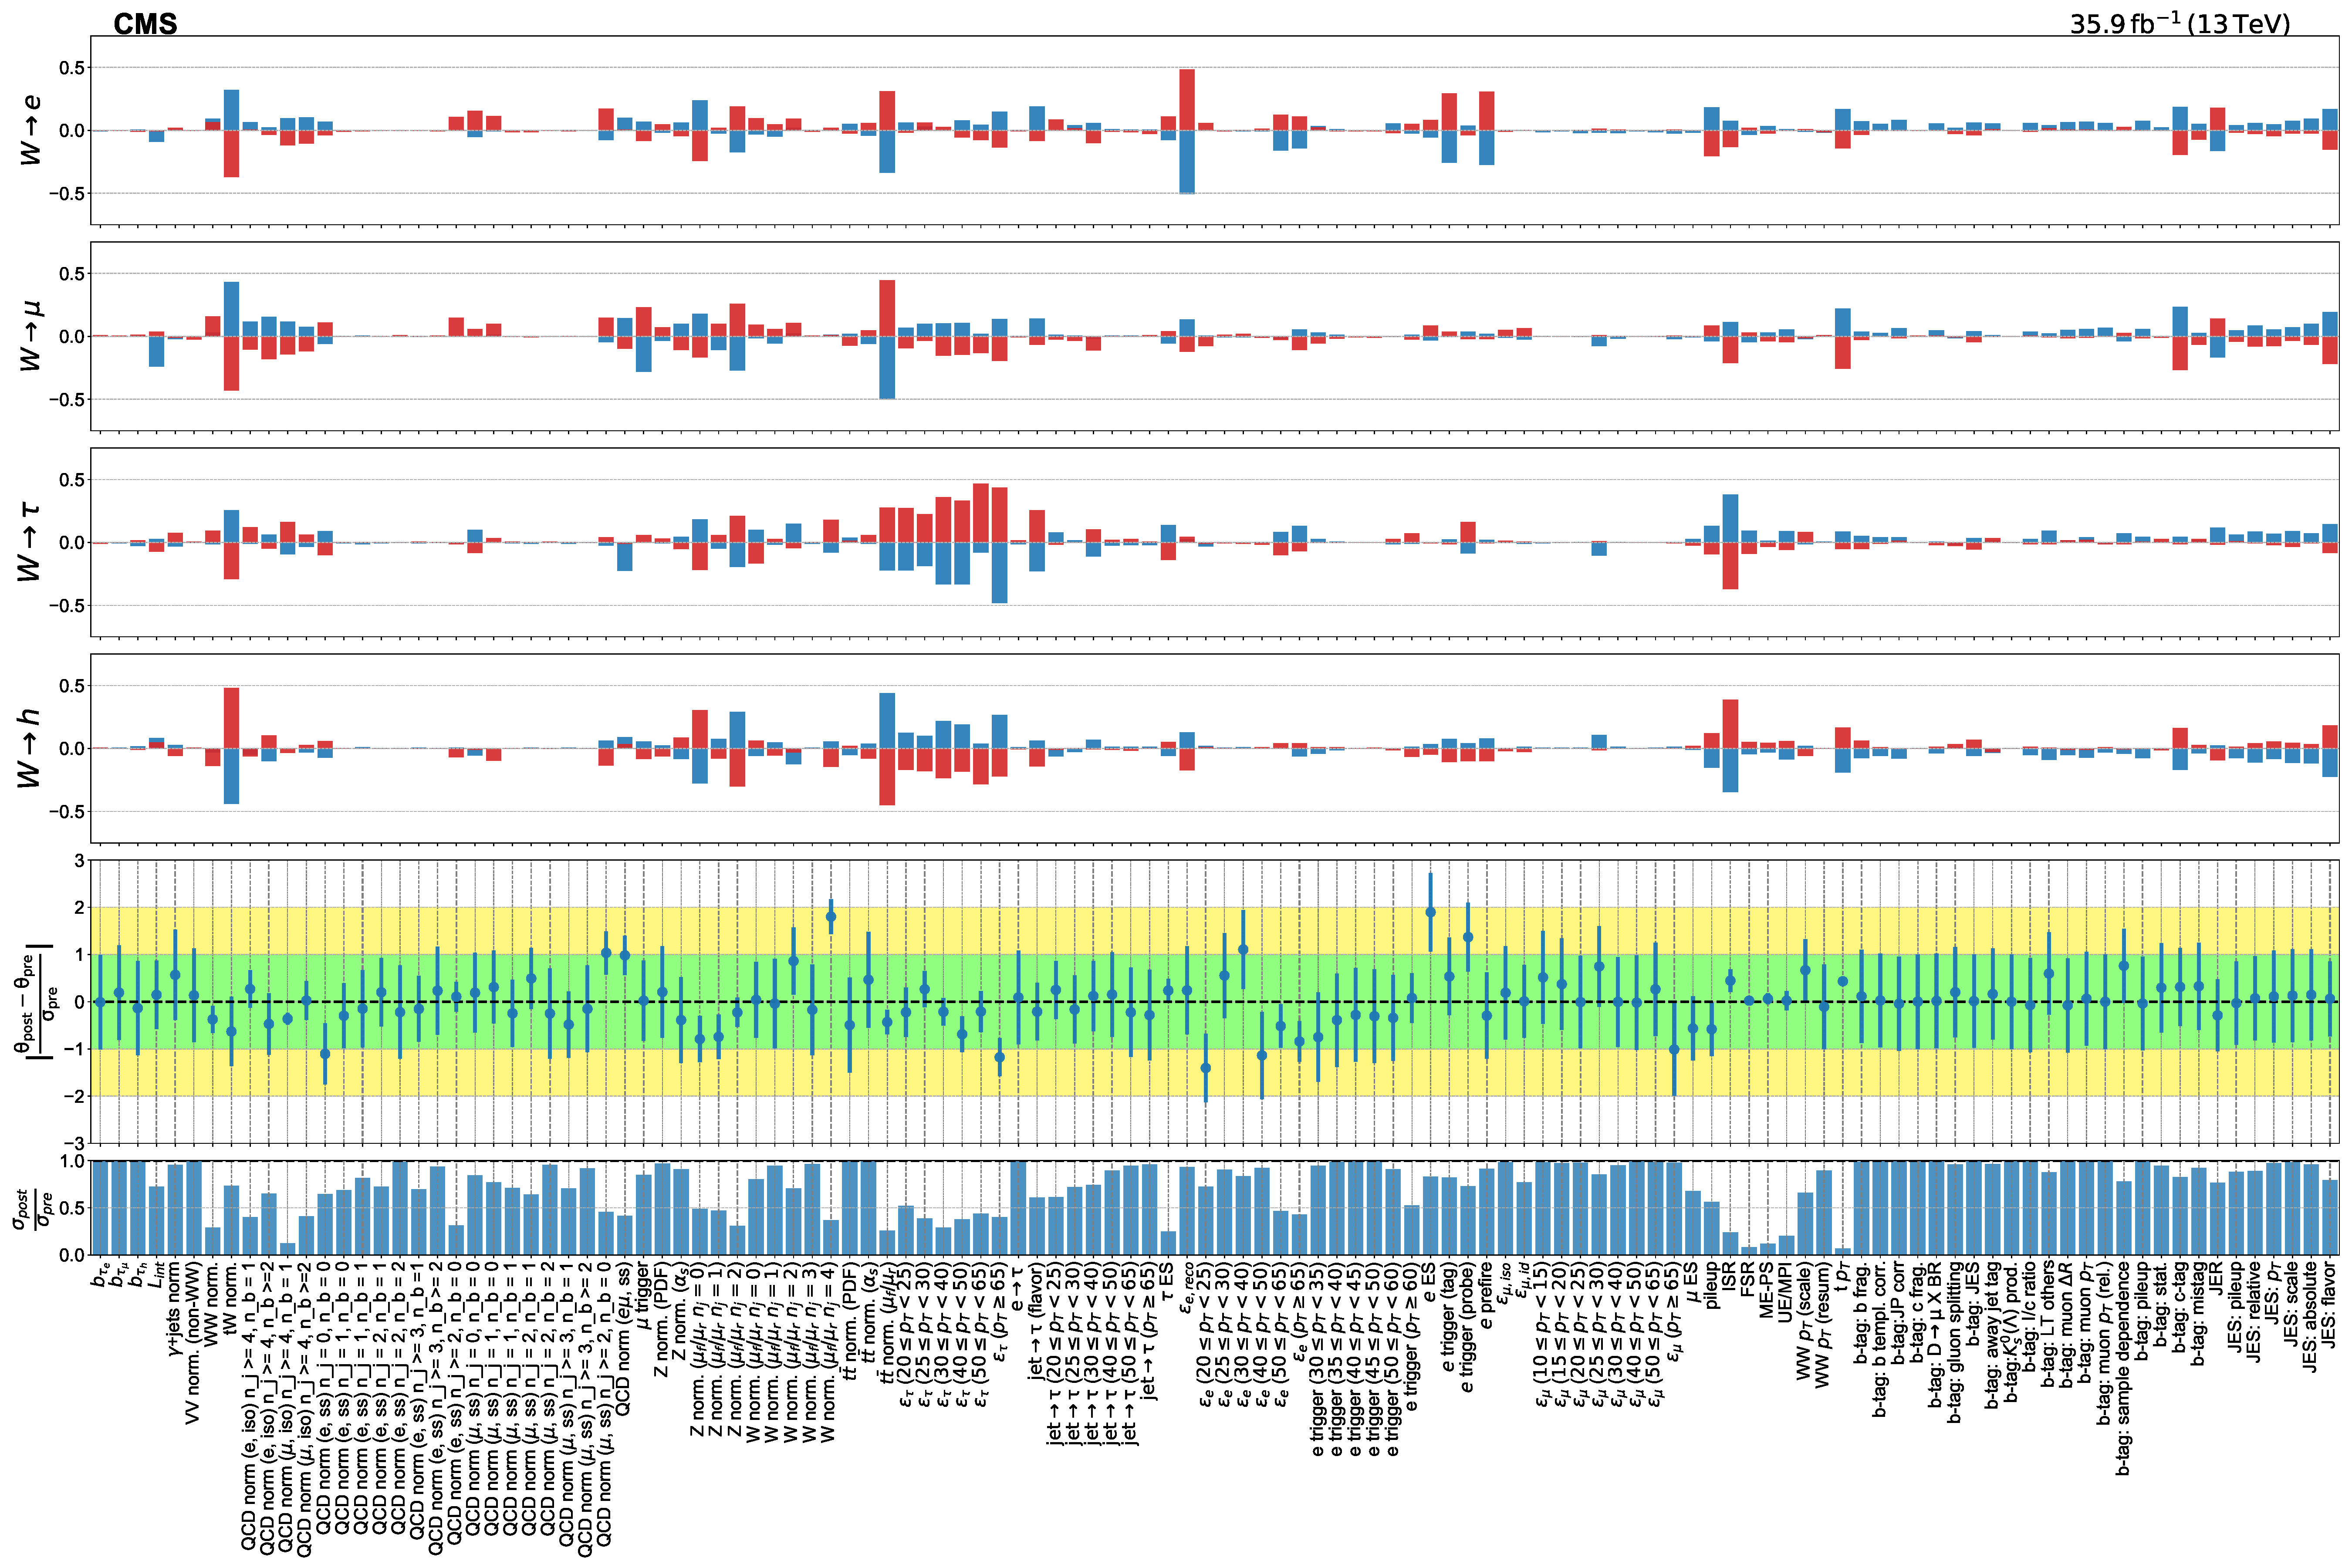
\includegraphics[width=\textwidth]{chapters/Analysis/sectionSystematics/figures/pulls_impacts_final.pdf}
\end{frame}









